\chapter{Introduction}
Due to the expansion of the universe, the farther galaxies are, the faster they appear to move. This relative motion causes the light that is emitted by these galaxies to be Doppler-shifted. The effect where the light is stretched due to the expansion is called cosmological redshift. Therefore, measurements of galaxy redshifts by missions such as Euclid can be used to determine their velocities, and by assuming a cosmology, the redshifts can be converted into distance measurements. This can be used to make a 3D map of the distribution of galaxies in the observable universe, giving insights into the large-scale structure formation and distribution of dark matter.

\begin{wrapfigure}{r}{0.5\textwidth}
    \vspace{-1em}   
	\centering
	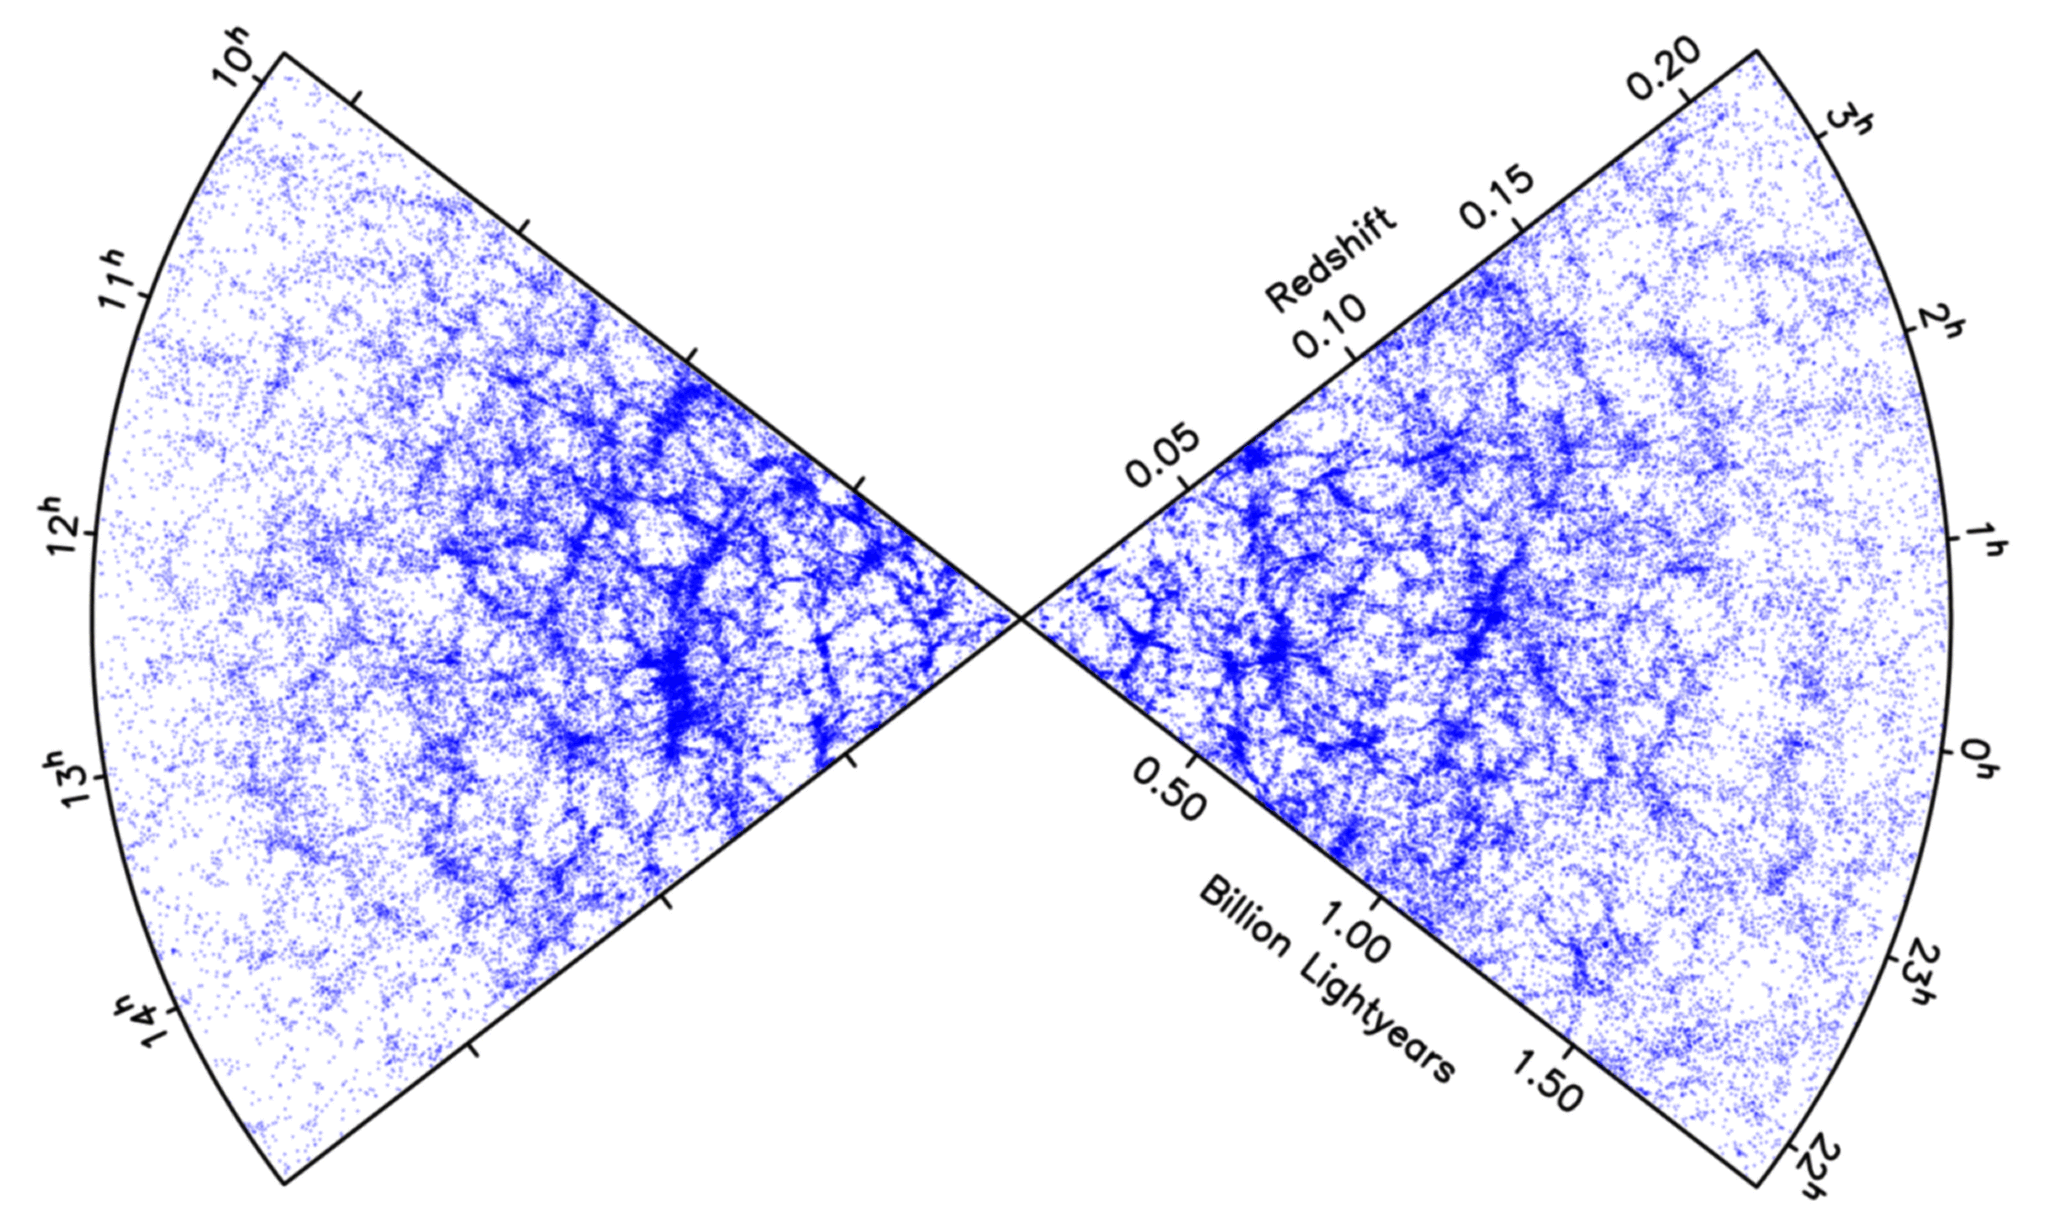
\includegraphics[width=0.9\linewidth]{results/figures/papers/2df_slice_blue_big.png}
	\caption{2dF redshift galaxy survey\protect\footnotemark}
    \label{fig:placeholder}
    %\vspace{-1ex}
\end{wrapfigure}
\footnotetext{\url{https://www.roe.ac.uk/~jap/2df/}}

% \begin{equation}
%     z = \frac{\Delta\lambda}{\lambda_\mathrm{emitted}}=\frac{\lambda_\mathrm{observed}-\lambda_\mathrm{emitted}}{\lambda_\mathrm{emitted}}
% \end{equation}
The most accurate measurements of the redshift are spectroscopic redshifts. This involves using spectroscopy to directly determine the redshift, for example, by examining shifts in specific atomic lines or other spectral features. The precision of determining the redshift using spectroscopy is \textbf{NUMBER} \citep{SourceNeeded}. However, there is a problem with this method. It can only be applied to thousands of objects at a time \citep{SourceNeeded}. Thus, this method takes considerably longer to determine the redshift for a larger number of sources, like the billions of galaxies in large surveys. Photometry can also be used to find the redshift for a large number of sources at the same time. Photometry is, in essence, spectroscopy with a low sampling resolution of the \gls{sed} of objects. Therefore, photometry can only reach accuracies of \textbf{NUMBER} \citep{SourceNeeded}, but it can be applied to a much larger number of sources at one time. Accurate colors require accurate photometry. However, current techniques have limitations in combining the information of different bands. This is where \gls{x-bap} comes in. This work develops \gls{x-bap}, which corrects the effects the \gls{psf} has on observations in different bands and applies aperture photometry to the pre-seeing image.

\section{Photometric colors}

Photometry is a method to determine the brightness of objects in the sky. The measurements use a broadband or narrowband filter, which only allows light in a certain wavelength range to pass through and be detected by the observer. The filter detects only a fraction of the light in the wavelength range, which is called the filter response curve. For example, Euclid has 4 different broadband filters that each operate at different wavelength regions as shown in \autoref{fig: Euclid filter response}.

\begin{figure}[H]
    \centering
    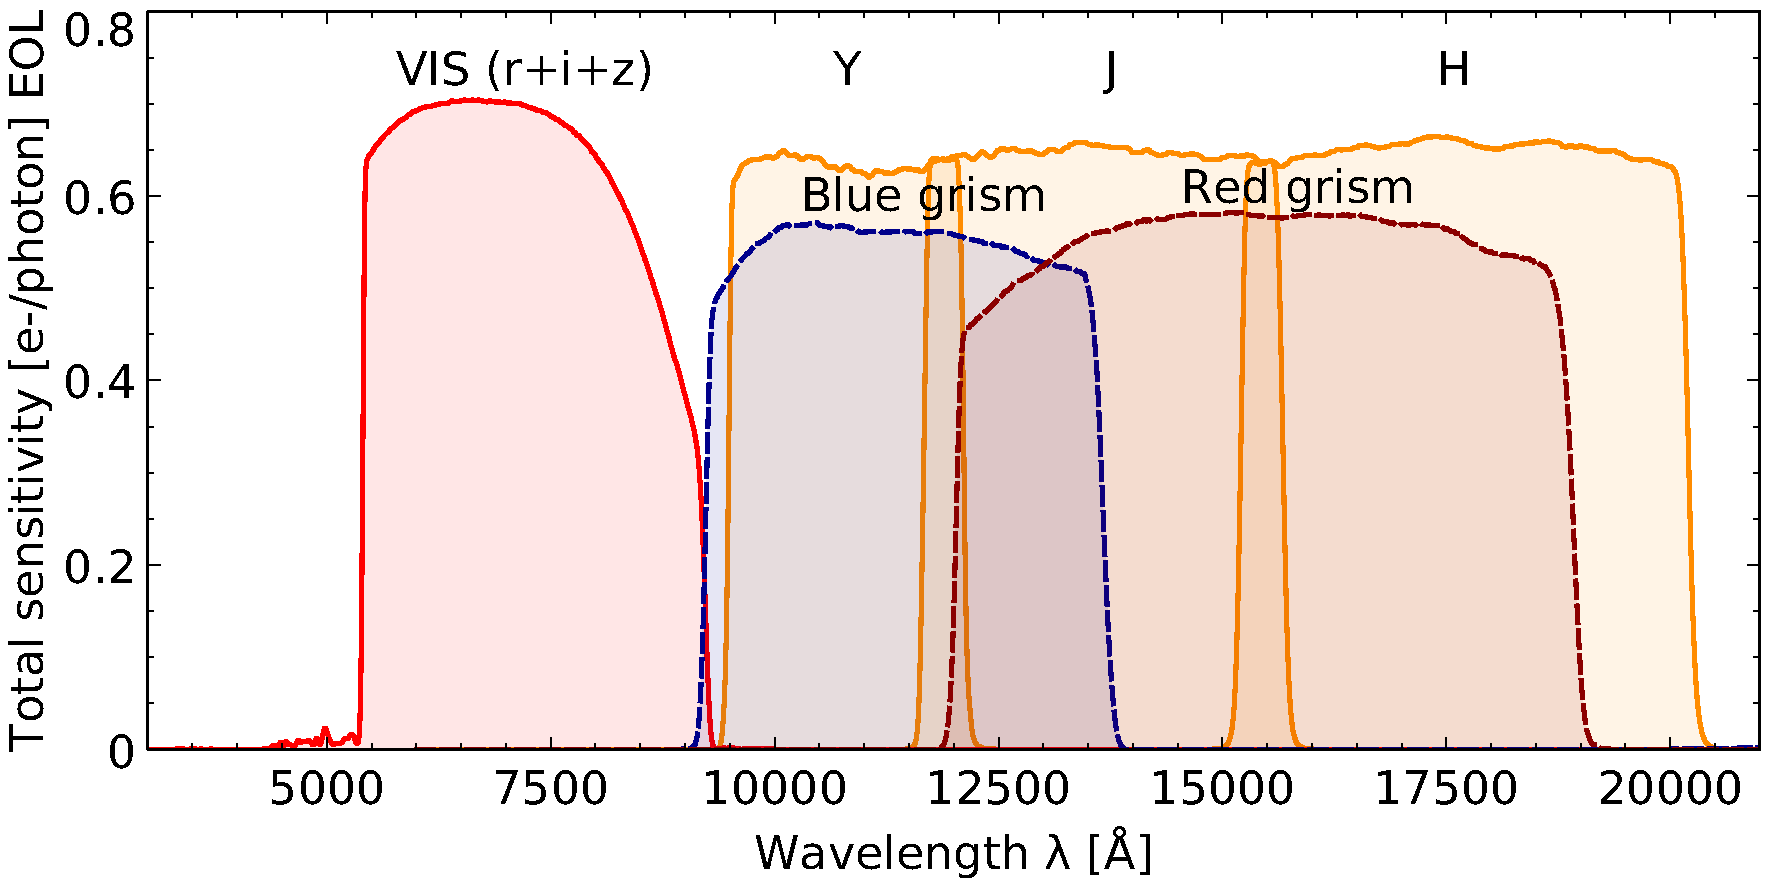
\includegraphics[width=0.8\linewidth]{results/figures/papers/Euclid.EOL.2020.pdf}
    \caption{The filter response curves for the photometric (solid lines) and spectroscopic bands (dashed lines) on board Euclid. The VIS band is part of the \gls{vis} instrument, whereas the Y-, J-, and H-bands are part of \gls{nisp}.  \citep{scaramella_euclid_2021}}
    \label{fig: Euclid filter response}
\end{figure}
The observed flux is the spectrum of the object integrated over the wavelengths 

\begin{equation}
    F_i^\mathrm{obs}=\int S(\lambda)T_i(\lambda)d\lambda,
\end{equation}
$S(\lambda)$ is the \gls{sed} of the observed sky and $T_i(\lambda)$ is the filter response curve of filter $i$. This quantity gives a sense for the total amount of flux in a specific wavelength range. 
The flux can be converted to an apparent magnitude. The lower the apparent magnitude of an object is, the brighter it is in the sky. The apparent magnitude of an object can be calculated using 

\begin{equation}\label{eq: magnitude}
    m_i=-2.5\log_{10}\left(F_i\right) + C
\end{equation}
where $F_i$ is the flux measured in the broadband $i$ and $C$ is the zeropoint, which can be chosen depending on the application of the measurements. The color of an object is the difference between the magnitudes of two different filters.

\begin{equation}
    (m_A-m_B)=-2.5\log_{10}\left(\frac{F_A}{F_B}\right)
\end{equation}
Colors are often denoted as the difference in the filters instead of the difference in the magnitude of the filter (e.g., $(A-B)$ means the same thing as $(m_A-m_B)$). Different magnitude systems define the value of $C$ in \autoref{eq: magnitude}. The Vega magnitude system defines the magnitude of the star Vega to be 0 in every filter. This way, you find that it gives the magnitude of an object
\begin{equation}
    m_i=-2.5\log\left(\frac{F_i}{F_i^\mathrm{Vega}}\right).
\end{equation}
However, there is a disadvantage to using this system as it requires knowledge of the spectrum of Vega and ...
An alternative system is the AB magnitude system, where the magnitude of a source is
\begin{equation}\label{eq: magnitude ab}
    m_\mathrm{AB}=-2.5\log_{10}\left(\frac{F_\nu}{3613 \mathrm{\;Jy}}\right).
\end{equation}
So the zero point of the AB magnitude system is independent of the wavelength, which makes it more accurate, as it does not depend on measurements of the colors of Vega. 

\section{Types of objects}
Large sky surveys capture the light of different types of astrophysical objects. These objects have different morphologies and, most importantly, \glspl{sed}. This means that accurate photometric color measurements can be used for classification of sources.  

\subsection{Stars}
Stars are a large collection of gas, mostly consisting of hydrogen and helium, which gets fused in the core of the star, producing energy. The \gls{sed} of stars can generally be approximated well by the spectrum of a blackbody. 

Due to their small apparent size in the sky, stars behave like point sources. This means that when they are observed, they take the shape of the \gls{psf}. This means that stars can be used to estimate the \gls{psf} in an image. 

Main sequence
HR-diagram

Bleeding blending saturation

\subsection{Galaxies}

Galaxies are collections of stars, gas, and dust residing in a dark matter halo. 

Generally, there are 2 types of galaxies: elliptical and spiral. Elliptical galaxies that the are elliptically shaped, whereas spiral galaxies are flat disks often with spiral arms. However, sometimes it is difficult to place some galaxies in either one of the two classes. These irregular galaxies are the  

Unlike stars, the apparent size of galaxies is larger, which means that they appear as extended objects in observations. Galaxies are brighter towards the center while the outer regions are fainter. This makes it difficult to find the total flux of galaxies. 

Galaxies do not form 

red galaxies that 
star-forming blue galaxies
and then green-valley galaxies in the transition between star-forming and dead. 

\subsection{QSOs}
\glspl{qso} are \glspl{agn}. These objects are \glspl{smbh} that reside at the center of galaxies. The black hole is accreting matter and can output the same power as \textbf{NUMBER} Suns. Due to this high luminosity, these objects also appear as point sources in observations. However, the spectrum of \glspl{qso} is much different, as they have a power-law continuum. 

% \subsection{Little Red Dots}



\section{Current techniques}

Photometry is used to find the intrinsic brightness of sources. Different methods have been developed for different applications, but no method is optimal for all applications. One of the main challenges with photometry is combining the information from different bands correctly. Observations have different pixel scales, different \glspl{psf}, seeing, etc., that can introduce inaccuracies in the flux measurements, which in turn make further analysis less accurate.

\subsection{Aperture Photometry}

Aperture photometry works by taking a weighted sum of pixel values in an observation. In its simplest form, circular aperture photometry, only the pixels within a circular aperture are summed together. More generally, the aperture can be a weighted aperture that gives different weights to pixel values before summing them together. This can be written like
\begin{equation}\label{eq: flux}
    F_\mathrm{A} = \sum_{x,y}O(x,y)W_\mathrm{A}(x,y),
\end{equation}
where $O(x,y)$ and $W_\mathrm{A}(x,y)$ are the pixel values of the observation and the values of the weighted aperture.

The advantages of aperture photometry are that it is easy to implement and quick. Furthermore, it works well for isolated sources. However, difficulties arise when comparing the flux of bands with very different-sized \glspl{psf}. As the observation with a larger \gls{psf} can result in the signal being outside of the aperture, whereas it is within the aperture for the band with the smaller \gls{psf}.

% \cite{merlin_-phot_2019}

\subsection{PSF-fitting Photometry}

In \gls{psf}-fitting photometry, sources are assumed to be point sources. This means that the observed image of a source is 
\begin{equation}
    O(x,y)=F\times PSF(x,y),
\end{equation}
where $F$ is the flux. So the flux can be directly computed by fitting the \gls{psf} to sources. This technique works great for stars, and even in crowded environments. However, a big limitation for this technique is extended sources. 

\subsection{Model-fitting Photometry}

Unlike \gls{psf}-fitting photometry, model-fitting photometry can be applied to extended sources. It works by using a model for the galaxy and convolving that with the \gls{psf}. By fitting the result to an observation, the flux can be estimated. This technique can find the total flux of a source and also find galaxy parameters. However, the model biases the result as galaxies are complex. This is especially true for irregular galaxies. Furthermore, the model fitting is computationally more expensive than a simpler method like aperture photometry.

% \cite{merlin_t-phot_2015}

\subsection{GAaP}\gls{gaap} has been implemented in KiDS and UNIONS
\cite{Kuijken_2008}

\section{New Technique}
This work introduces a different way of measuring the flux of objects in an image, \gls{x-bap}. This method compensates for the effects the \gls{psf} and seeing have on the image, which allows for more accurate colors by combining flux measurements in different bands.  


\section{Scope}

The goal of this thesis is to explore a new method of determining the colors of objects, \gls{x-bap}, apply that technique to survey observations of Euclid, and determine the photometric redshift of objects. 

First, the algorithm is explained. Subsequently, the method's limitations and accuracy are evaluated using simulations. Next, this method is applied to Euclid images. Lastly, the colors determined with \gls{x-bap} are used to categorize the sources. 
\newpage